% ELEC-VQA public manuscript, IEEE Access class.
\documentclass{ieeeaccess}
\usepackage{cite}
\usepackage{amsmath,amssymb,amsfonts,graphicx,booktabs,tabularx,array,xspace}
\usepackage{textcomp}
\usepackage{placeins}
\usepackage{needspace}
\definecolor{draftgray}{gray}{0.45}
\definecolor{RQBackground}{rgb}{0.94,0.97,0.99}
\definecolor{RQInk}{rgb}{0.0,0.35,0.55}
\def\thevol{--}
\def\theyear{--}
\usepackage[hidelinks]{hyperref}
\hypersetup{pdftitle={Improving Electrical Schematic Understanding with the ELEC-VQA Dataset: A Comparative Study}}
\setlength{\emergencystretch}{2em}
\newcommand{\dataset}{ELEC-VQA\xspace}
\newcommand{\pending}{\phantom{00.00}}
\newcommand{\fillhere}[1]{}
\newcommand{\resultslot}[1]{\fillhere{#1}}
\newcommand{\figspace}[2]{\fbox{\parbox[c][#1][c]{.94\linewidth}{\mbox{}}}}
\newcommand{\researchquestion}[3]{\par\smallskip\noindent\colorbox{RQBackground}{\parbox{\dimexpr\linewidth-2\fboxsep\relax}{\textcolor{RQInk}{\textbf{#1. #2}}\par\smallskip #3}}\par\smallskip}
\begin{document}
\history{}
\doi{}
\title{Improving Electrical Schematic Understanding with the ELEC-VQA Dataset: A Comparative Study}
\author{\phantom{Author name}}
\address{\phantom{Affiliation}}
\corresp{\phantom{Corresponding author}}

\markboth{ELEC-VQA: Electrical Schematic Understanding}{ELEC-VQA: Electrical Schematic Understanding}
\begin{abstract}
Electrical schematic interpretation requires models to associate terminal labels with conductors, distinguish wiring topology from contact state, and justify conclusions under explicit operating assumptions. Existing visual question answering benchmarks provide limited coverage of this combination in native engineering drawings. This article introduces ELEC-VQA, a source-traceable dataset constructed from computer-aided design drawings of substation secondary circuits. The dataset contains 10,201 English question--answer records across 15 task families and 1,019 image configurations, comprising 300 original local windows and 719 controlled drawing variants. Each record couples a concise answer with compact evidence and executable checks over a bounded terminal graph. Native rendering preserves conductor geometry, while source-disjoint partitions reduce leakage between related questions and edited drawings. Two aligned supervision views enable a controlled comparison of answer-only and evidence-guided fine-tuning of a seven-billion-parameter vision--language model. A comparative study evaluates three general-purpose vision--language model families and two aligned adaptations of a 7B backbone. With provisional reference-based supplementary adjudication of unscored outputs, answer-only fine-tuning increases direct-answer accuracy from 37.16\% to 74.27\%. Under common explanation prompting, evidence-guided fine-tuning achieves 64.24\% joint answer--evidence correctness, compared with 46.17\% for answer-only supervision, while their answer accuracies are 67.97\% and 70.16\%. Evidence support among correct answers and controlled-change analyses reveal selective benefits for multi-condition reasoning and measurement planning, alongside weaknesses in state invariance and visual topology changes. ELEC-VQA enables evaluation of both electrical decisions and their explicit support, without equating generated explanations with faithful internal reasoning.

\end{abstract}
\begin{keywords}
Chain-of-thought supervision, electrical schematics, engineering datasets, evidence-grounded reasoning, parameter-efficient fine-tuning, visual question answering.
\end{keywords}
\titlepgskip=-15pt
\maketitle
\section{Introduction}\label{sec:introduction}
Electrical schematics encode engineering decisions through relations among terminals, conductors, contacts, and devices. During drawing inspection or maintenance preparation, an engineer may need to determine whether opening a contact disconnects a branch, identify faults consistent with continuity readings, or assess whether a proposed connection satisfies a stated requirement. These questions depend on the interaction between visible topology and explicitly specified conditions. Correct recognition of component names alone is insufficient: overlooking a short conductor, assuming an unsupported junction, or confusing an unknown contact state with a closed contact can reverse the answer.

Figure~\ref{fig:introcase} illustrates this challenge through a measurement-planning record associated with an original DWG circuit window in \dataset. Given three candidate single-contact faults, the task is to choose the fewest continuity measurements that distinguish their outcomes. The upstream contact is common to the relevant branches, whereas the two downstream contacts affect different branches. Measurements at 1DK6:4 and JD1:1 therefore distinguish an upstream interruption from the two branch-specific faults. The model must combine terminal grounding, wiring topology, and explicit fault assumptions before selecting these informative test points. The compact fault-signature table explains both why two tests suffice and why a single binary measurement cannot suffice. This example motivates annotations that supervise an engineering decision together with a checkable justification, rather than label recognition alone.

\begin{figure*}[t]
\centering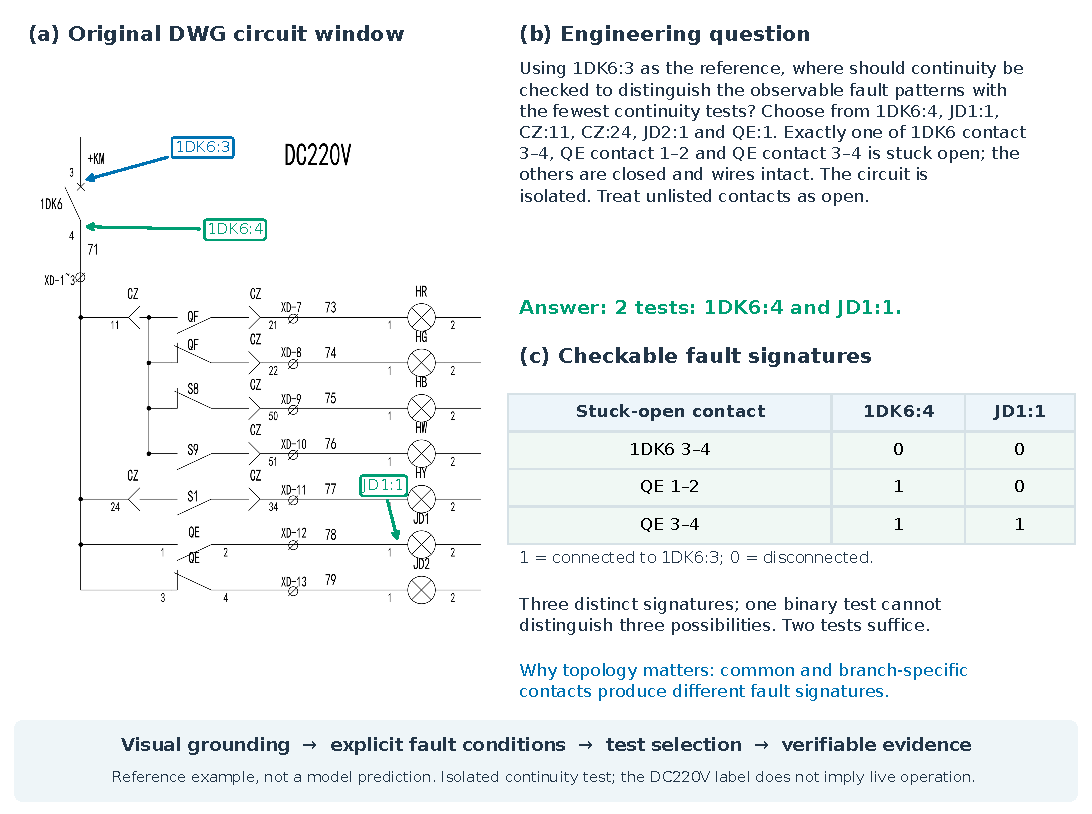
\includegraphics[width=\textwidth]{assets/figure_01.pdf}
\caption{An illustrative \dataset measurement-planning example from the training partition, using an original DWG window. The released question and answer appear beside compact reference evidence. Continuity tests at 1DK6:4 and JD1:1 give distinct signatures $(0,0)$, $(1,0)$, and $(1,1)$ for the three candidate faults; a single binary measurement cannot distinguish all three. Rendering adjustments and editorial callouts preserve the original wiring topology. The associated graph queries verify the stated fault signatures.}
\label{fig:introcase}
\end{figure*}

Visual question answering (VQA) offers a natural-language interface to this information. Document-oriented benchmarks establish the importance of reading text within its visual context~\cite{singh2019textvqa,mathew2021docvqa}, while diagram and chart benchmarks examine relations that cannot be recovered from isolated labels~\cite{kembhavi2016diagram,masry2022chartqa}. Recent engineering benchmarks extend this direction toward professional artifacts. DrawingVQA evaluates construction drawings through perceptual, contextual, and domain-expert questions~\cite{jung2026drawingvqa}; DesignQA examines engineering requirements and documentation~\cite{doris2025designqa}; and MechVQA addresses mechanical drawing interpretation~\cite{kou2026mechvqa}. Together, these studies motivate task definitions grounded in engineering practice rather than generic image description.

Electrical diagram understanding is itself an established research area. CircuitVQA, ElectroVizQA, and EEE-Bench cover circuit images, educational electronics, and broader electrical engineering problems, respectively~\cite{mehta2024circuitvqa,meshram2024electrovizqa,li2025eeebench}. CircuitSense studies visual-to-symbolic circuit analysis~\cite{akbari2025circuitsense}, and OmniSch evaluates schematic grounding and graph construction~\cite{lu2026omnisch}. The complementary question considered here is how to construct reusable training and evaluation data for local engineering decisions in native electrical drawings, with inspectable evidence and reproducible state-dependent labels.

Three requirements follow. First, annotations must connect a natural-language conclusion to identifiable visual and electrical entities. A plausible explanation is insufficient unless its stated route, blocking condition, or diagnostic alternative can be checked. Second, the question must distinguish what is drawn from what is assumed. A static schematic does not establish the present voltage or operating state of equipment. Third, evaluation must account for dependencies among questions, overlapping windows, and edited versions of the same source circuit. Treating these observations as independent can overstate generalization to unseen engineering documents.

We address these requirements through \dataset, a dataset derived from native computer-aided design (CAD) drawings. The dataset comprises 10,201 English QA records over 1,019 image configurations, sourced from 44 DWG files across 14 substation projects. Its 300 original context windows and 719 controlled native-DWG variants support tasks involving conditional connectivity, diagnostic ambiguity, measurement selection, and bounded design checks. A short evidence sequence accompanies each answer, while terminal identifiers, source geometry, and executable graph queries retain the underlying verification record. The graph is used to construct and check annotations; it is not supplied as an input to the image-question model.

The dataset also enables a controlled comparison of supervision strategies. We fine-tune the same seven-billion-parameter vision--language backbone with either short answers alone or compact evidence followed by the same answers. Low-rank adaptation (LoRA)~\cite{hu2021lora} provides a standard implementation of domain adaptation. Evidence-guided chain-of-thought denotes externally checkable intermediate statements; it does not imply access to hidden computation or a separately established teacher-distillation process. The empirical objective is to determine where this supervision is beneficial, neutral, or detrimental, rather than to assume a uniform advantage.

The contributions are threefold:
\begin{enumerate}
\item A CAD-derived electrical schematic dataset with 15 task families, concise English questions and answers, compact evidence, and terminal-level provenance.
\item A construction and verification protocol combining native rendering, controlled wiring interventions, executable checks, and source-disjoint partitions.
\item A comparative study design separating general-model benchmarking, controlled answer/evidence supervision, semantic answer correctness, and evidence validity.
\end{enumerate}
The scope is electrical schematic understanding within substation secondary wiring; broader electrical-domain transfer is an empirical question. Section~\ref{sec:related} situates the resource, Section~\ref{sec:dataset} describes its construction, and Sections~\ref{sec:protocol} and~\ref{sec:experiments} specify the comparison and evaluation.

\section{Related Work}\label{sec:related}
\subsection{Document and Diagram Question Answering}
TextVQA introduces questions requiring recognition and contextual use of text in images~\cite{singh2019textvqa}. DocVQA transfers question answering to document pages, where layout and structure determine how textual evidence should be interpreted~\cite{mathew2021docvqa}. ChartQA and InfographicVQA extend the problem to joint interpretation of text, graphics, and quantitative relations~\cite{masry2022chartqa,mathew2022infographic}. These resources establish that reading and reasoning should be assessed together, but their document semantics differ from the conductor and contact relations of an electrical drawing.

AI2D represents diagram elements and their relations for diagram understanding~\cite{kembhavi2016diagram}. GQA uses structured scene representations to generate compositional questions and evaluate consistency~\cite{hudson2019gqa}. These approaches motivate explicit representations and relational checks, although a scene graph does not by itself express electrical continuity under changing contact states. MMMU provides a broader test of multimodal subject knowledge, including engineering~\cite{yue2024mmmu}; a specialized benchmark is needed to resolve failures at individual terminals and connections.

\subsection{Engineering Drawings and Professional Questions}
DrawingVQA is closely related in its use of authentic engineering drawings and professionally meaningful questions~\cite{jung2026drawingvqa}. Its construction-drawing benchmark contains 33 drawings and 92 curated QA pairs, organized by reasoning depth and by engineering and model-capability dimensions. This motivates separating recognition from contextual and engineering judgement. Our setting differs in the target artifact and verification mechanism: electrical continuity and explicit state interventions are represented through bounded CAD-derived graphs. We do not compare benchmark accuracy across these different datasets or equate automatic labels with expert-authored annotations.

DesignQA connects engineering documentation, visual artifacts, and requirement checking~\cite{doris2025designqa}. Its emphasis on applying requirements is relevant to our bounded design-check tasks, where requirements are stated in the question rather than inferred from an unstated standard. Work in IEEE Access on multimodal document segmentation further links technical QA to the organization of local visual elements~\cite{lvov2026segmentation}; our benchmark supplies a fixed local image rather than evaluating document retrieval. MechVQA combines mechanical drawings with recognition, reasoning, and judging tasks and domain adaptation~\cite{kou2026mechvqa}. These studies support a dataset-centered comparative design: the contribution lies in the representation of domain decisions, annotation provenance, and diagnostic evaluation, not merely in the number of image-question pairs.

\subsection{Electrical Schematics and Circuit Reasoning}
Earlier graph-based circuit-sketch recognition addresses the structured interpretation of drawn circuit elements~\cite{liu2020circuitsketch}. CircuitVQA addresses components, values, junctions, and positions in circuit images~\cite{mehta2024circuitvqa}. ElectroVizQA focuses on digital electronics problems~\cite{meshram2024electrovizqa}, whereas EEE-Bench spans multiple electrical and electronic engineering subdomains~\cite{li2025eeebench}. CircuitSense emphasizes deriving symbolic circuit models from visual inputs~\cite{akbari2025circuitsense}; OmniSch focuses on grounding schematic entities and recovering spatially weighted netlist graphs~\cite{lu2026omnisch}. Work on near-sight correction further considers local visual inspection in circuit understanding~\cite{kulkarni2025nsc}. These directions show why a response-level score alone cannot localize whether an error arose from reading, topology extraction, or subsequent reasoning.

\dataset complements these resources with native industrial wiring images, explicit contact assumptions, and brief verifiable explanations. Its tasks concern visible external connections, not unrestricted analog simulation, complete device behavior, or undocumented internal wiring. Table~\ref{tab:related} summarizes the scope and verification emphasis of these resources; it is a descriptive comparison rather than a cross-dataset performance ranking.

\begin{table*}[t]
\centering\small
\caption{Related resources and their reported emphasis. Descriptions concern their task definitions, not results from a common evaluation.}
\label{tab:related}
\begin{tabularx}{\textwidth}{@{}p{23mm}XXXX@{}}\toprule
Resource & Source artifact & Question emphasis & Evidence/verification & Evaluation unit \\\midrule
DrawingVQA~\cite{jung2026drawingvqa} & Construction drawings & Perception to expert judgement & Expert-curated QA / reasoning-depth labels & Drawing / question \\
DesignQA~\cite{doris2025designqa} & Engineering documents and visual artifacts & Requirements and compliance & Document-grounded references & Requirement / question \\
MechVQA~\cite{kou2026mechvqa} & Mechanical drawings & Recognition, reasoning, judging & Semi-automated quality-control pipeline & Drawing / question \\
CircuitVQA~\cite{mehta2024circuitvqa} & Circuit images & Components, values, junctions, positions & Circuit-specific QA annotations & Image / question \\
EEE-Bench~\cite{li2025eeebench} & Electrical/electronics problems & Broad engineering problem solving & Curated problem references & Problem \\
CircuitSense~\cite{akbari2025circuitsense} & Schematics and block diagrams & Perception, analysis, design & Symbolic-equation references & Problem / hierarchy \\
OmniSch~\cite{lu2026omnisch} & PCB schematic diagrams & Grounding and graph construction & Entity / netlist graph annotations & Diagram / structured task \\
\dataset & Native substation DWGs & State-dependent local wiring decisions & CAD graph checks + compact certificates & QA / image; source-grouped split \\
\bottomrule\end{tabularx}
\end{table*}

\subsection{Evidence Supervision and Evaluation}
ScienceQA studies multimodal questions with explanatory supervision~\cite{lu2022scienceqa}, and A-OKVQA provides knowledge-based visual questions with rationales~\cite{schwenk2022aokvqa}. Multimodal-CoT separates rationale generation and answer inference~\cite{zhang2024multimodalcot}; Distilling Step-by-Step uses teacher-generated rationales to supervise smaller language models~\cite{hsieh2023distilling}. These results motivate an investigation of intermediate supervision, but do not establish that additional explanatory tokens improve every schematic task. Our evidence originates from CAD graphs and rules, rather than a documented large-model teacher.

Explanation evaluation requires a separate notion of support. Multimodal explanation research distinguishes textual justification from visual evidence~\cite{park2018explanations}, and ERASER distinguishes rationale alignment from faithfulness~\cite{deyoung2020eraser}. DRAGON evaluates evidence localization over diagrams with the correct answer supplied~\cite{iyengar2026dragon}; our primary task instead requires predicting the answer from an image and question. Generated reasoning may also omit factors that actually influenced a prediction~\cite{turpin2023unfaithful}. We therefore evaluate explicit evidence as a checkable solution certificate, without treating fluent prose as proof of internal reasoning.

Visual instruction tuning and modern open vision--language backbones provide the implementation basis~\cite{liu2023llava,bai2025qwen,li2024onevision}. Position, verbosity, and self-preference effects documented for language-model judges~\cite{zheng2023judge} motivate blinded scoring, structured references, and independent reliability checks.

For generative VQA, LAVE replaces exact string agreement with reference-guided answer assessment~\cite{manas2024lave}. Qwen2.5-32B-Instruct has also been evaluated as an instruction-model judge baseline in prior research~\cite{yu2025risejudge}. We adopt reference-guided assessment with explicit electrical criteria for terminal identities, contact conditions, solution completeness, and admissible alternatives. This is a domain adaptation of the evaluation paradigm; prior judge benchmarks do not establish reliability on electrical drawings, which requires independent human calibration.

Semantic text metrics such as BERTScore compare contextual token representations rather than exact word identity~\cite{zhang2020bertscore}. Electrical QA additionally requires explicit assessment of terminal identities and state-dependent conclusions. G-Eval provides a structured rubric-based evaluation framework~\cite{liu2023geval}, while LLMBar shows that persuasive style can mislead evaluators assessing instruction compliance~\cite{zeng2024llmbar}. Together, these studies motivate domain-specific scoring criteria and validation of evaluator decisions, rather than treating generic textual similarity as a complete measure of electrical correctness.

\section{ELEC-VQA Dataset Construction}\label{sec:dataset}
\subsection{Sources, Scope, and Sampling Units}
The ELEC-VQA dataset contains 10,201 QA records from 44 DWGs in 14 substation projects. Its 1,019 image configurations comprise 300 original local context windows and 719 controlled native-DWG variants. Original windows include surrounding schematic context and can overlap within a source drawing. Each record retains project, drawing, parent-window, and image-configuration identities, allowing dependent observations to be grouped during partitioning and analysis.

The intended unit of model input is a readable local schematic, rather than a complete drawing sheet. Selection favors windows whose visible external wiring and explicit contact pairs admit a bounded representation. Questions are not restricted to label transcription, but symbol and label recognition remain prerequisites for higher-level tasks. Figure~\ref{fig:pipeline} shows the construction overview, and Table~\ref{tab:splits} reports the partition summary.

\begin{figure*}[t]
\centering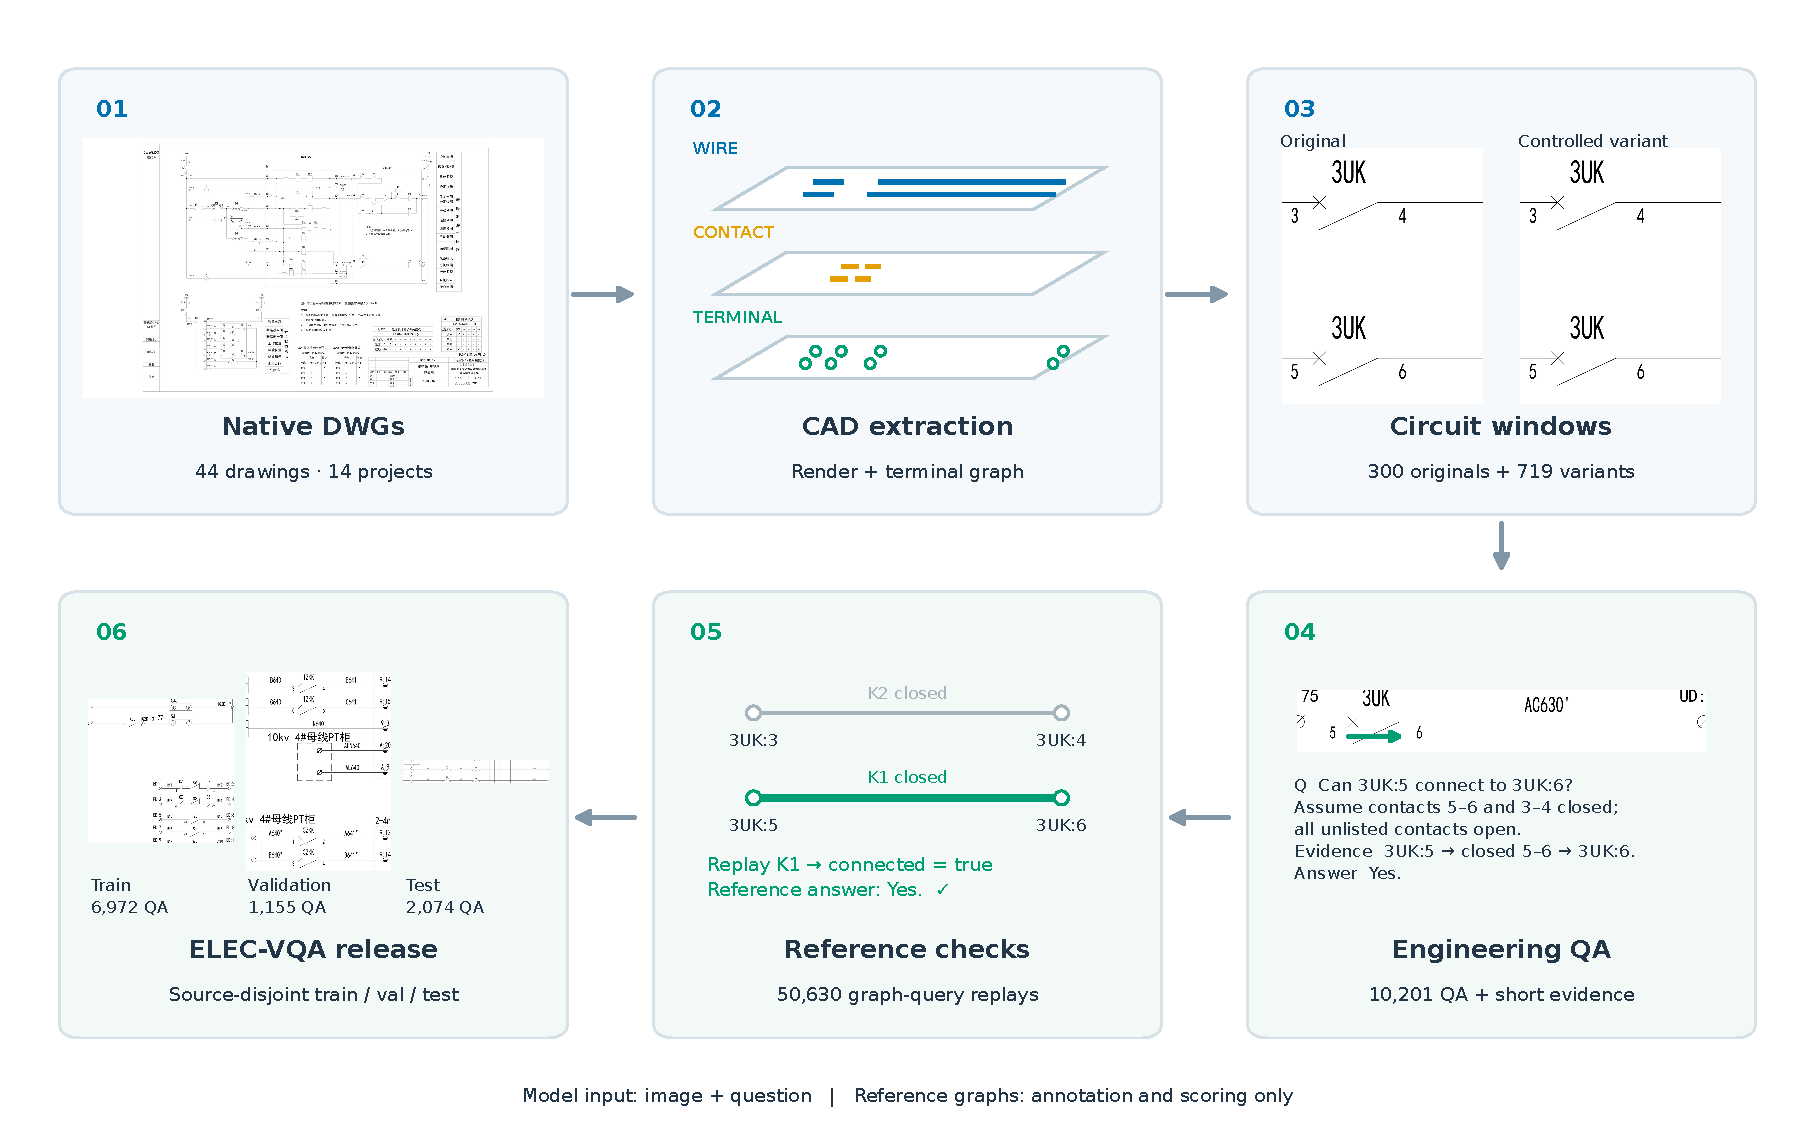
\includegraphics[width=\textwidth]{assets/figure_02.pdf}
\caption{Source-traceable dataset construction. The model receives an image and a question; source graphs and verification queries remain annotation-side information. }
\label{fig:pipeline}
\end{figure*}

\begin{table}[t]
\centering\small\setlength{\tabcolsep}{3pt}
\caption{Source-disjoint partitions. Windows count original contexts; variants count controlled native edits.}
\label{tab:splits}
\begin{tabular}{@{}lrrrrrr@{}}\toprule
Split & Proj. & DWGs & Windows & Variants & Images & QA \\\midrule
Train & 11 & 29 & 218 & 479 & 697 & 6,972 \\
Validation & 1 & 8 & 34 & 88 & 122 & 1,155 \\
Test & 2 & 7 & 48 & 152 & 200 & 2,074 \\
\midrule
Total & 14 & 44 & 300 & 719 & 1,019 & 10,201 \\
\bottomrule\end{tabular}
\end{table}

\subsection{Native Rendering and Source Traceability}
Extraction and rendering use the AutoCAD ActiveX COM interface. Rendering adjusts lineweight while preserving conductor geometry. Geometry entities are assigned a 0.35-mm lineweight without changing their coordinates. Rendering uses font-repaired companion working copies and project-specific plotting settings to produce native vector PDFs, which are rasterized and cropped using the recorded CAD-to-image mapping. This is distinct from raster dilation or generative redrawing. Lineweight adjustment is restricted to rendering; conductor coordinates and junction topology are preserved.

Terminal positions, conductor geometry, source identifiers, crop bounds, and image hashes support traceability. Controlled faults are applied in native working copies and rendered under registered views. Figure~\ref{fig:visual} shows registered crops from an original window and a controlled cross-network link, with their reference graphs. Display crops are distinguished from the full released images supplied to models.

\begin{figure*}[t]
\centering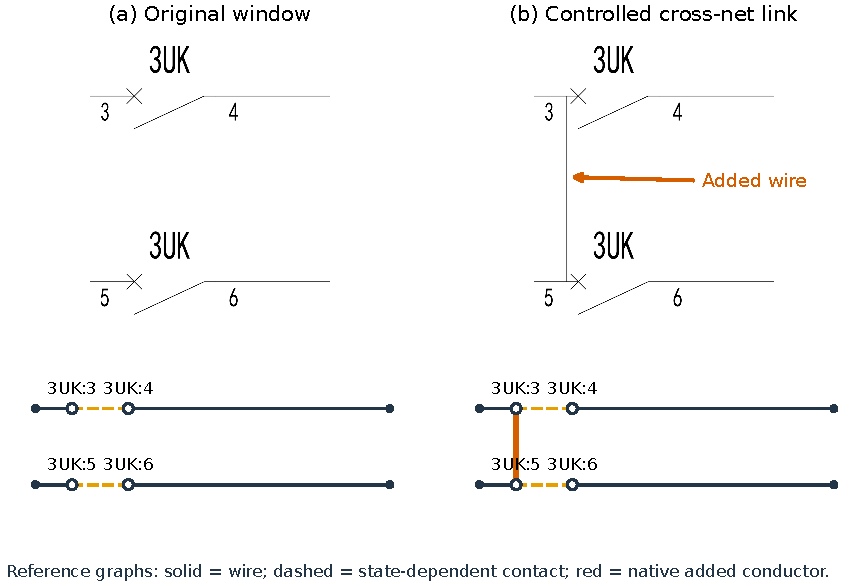
\includegraphics[width=.96\textwidth]{assets/figure_03.pdf}
\caption{Original local window and controlled native-DWG cross-network link. Registered crops show the added conductor connecting 3UK:3 and 3UK:5; the bottom panels show the corresponding bounded reference graphs. Dashed graph edges denote modeled contacts whose states are given by the question. Cropping and the arrow are for display only; models use the full released images.}
\label{fig:visual}
\end{figure*}

\subsection{State-Dependent Electrical Representation}
A local circuit is represented as $G=(V,E_w,E_c)$, where $V$ contains terminals and junctions, $E_w$ contains external conductors, and $E_c$ contains explicitly modeled contact pairs. For a state assignment $s$, removed-wire set $R$, and optional jumper set $J$, the active graph is
\begin{equation}
G_{s,R,J}=\left(V,(E_w\setminus R)\cup\{e\in E_c:s(e)=1\}\cup J\right).
\label{eq:active}
\end{equation}
Reachability in this graph determines bounded continuity. A contact's drawn appearance is not substituted for the state stipulated in the question. For a relevant unknown state, admissible assignments are evaluated separately; the answer may depend on that state. A graphical crossing is not automatically a junction, and undocumented device internals are excluded.

The representation does not establish actual voltage, current magnitude, protection operation, or system safety. Diagnosis assumes the stated fault family, and continuity measurements refer to isolated circuits with intact wires unless otherwise specified. These restrictions make the answer checkable; they also delimit the engineering claim.

\subsection{Questions, Answers, and Compact Evidence}
Fifteen task families cover conditional connectivity (T01), minimum closure (T02), wire groups (T03), contact-opening effects (T04), unknown states (T05), bypasses (T06), fault candidates (T07), measurement selection (T08), stated design requirements (T09), repair checks (T10), path order (T11), contact-network relationships (T12), diagnostic sufficiency (T13), voltage-information sufficiency (T14), and branch interruption (T15). Table~\ref{tab:tasks} reports their distribution. This is a task taxonomy, not fifteen independently validated levels of difficulty.

\begin{table}[t]
\centering\small\setlength{\tabcolsep}{3pt}
\caption{QA counts by task and split. T14 is a diagnostic control, and T12 contains no verified parallel cases.}
\label{tab:tasks}
\begin{tabularx}{\linewidth}{@{}lXrrrr@{}}\toprule
ID & Task family & Train & Val. & Test & Total \\\midrule
T01 & Connectivity & 1,495 & 259 & 440 & 2,194 \\
T02 & Minimum closure & 666 & 103 & 181 & 950 \\
T03 & Wire groups & 697 & 122 & 200 & 1,019 \\
T04 & Opening effects & 665 & 103 & 181 & 949 \\
T05 & Unknown states & 665 & 103 & 181 & 949 \\
T06 & Bypass analysis & 665 & 103 & 181 & 949 \\
T07 & Fault candidates & 471 & 58 & 127 & 656 \\
T08 & Measurement plan & 467 & 58 & 127 & 652 \\
T09 & Requirements & 697 & 122 & 200 & 1,019 \\
T10 & Repair checks & 130 & 24 & 69 & 223 \\
T11 & Path order & 164 & 30 & 57 & 251 \\
T12 & Contact relations & 60 & 20 & 40 & 120 \\
T13 & Diagnosis sufficiency & 60 & 20 & 40 & 120 \\
T14 & Voltage sufficiency & 10 & 10 & 10 & 30 \\
T15 & Branch interruption & 60 & 20 & 40 & 120 \\
\midrule Total & & 6,972 & 1,155 & 2,074 & 10,201 \\
\bottomrule\end{tabularx}
\end{table}

Questions use circuit-aware templates and controlled wording variants. Their language is English except where a source annotation must be quoted. A single image supports different decisions rather than repeated paraphrases counted as new semantic cases. Each master record separates the short answer, typed result, compact evidence steps, source entities, and verification queries. The evidence states the relevant condition, a conducting route or blocking fact, and only the alternatives necessary to justify the conclusion. Paths are certificates for positive reachability; negative statements retain the solver's reachable region in the structured record rather than claiming that an omitted route proves disconnection.

Evidence text is limited to 192 tokens under the local Qwen tokenizer, excluding headings and the answer; the published maximum is 189 and the mean is 39.63. Over-budget candidates are excluded rather than truncated. Figure~\ref{fig:distribution} shows the task, evidence-length, and image-provenance distributions. T12 currently contains series and separate-network cases but no verified parallel examples. T14 contains only negative sufficiency answers and is treated as a diagnostic control, not evidence of learned visual reasoning.

\begin{figure*}[t]
\centering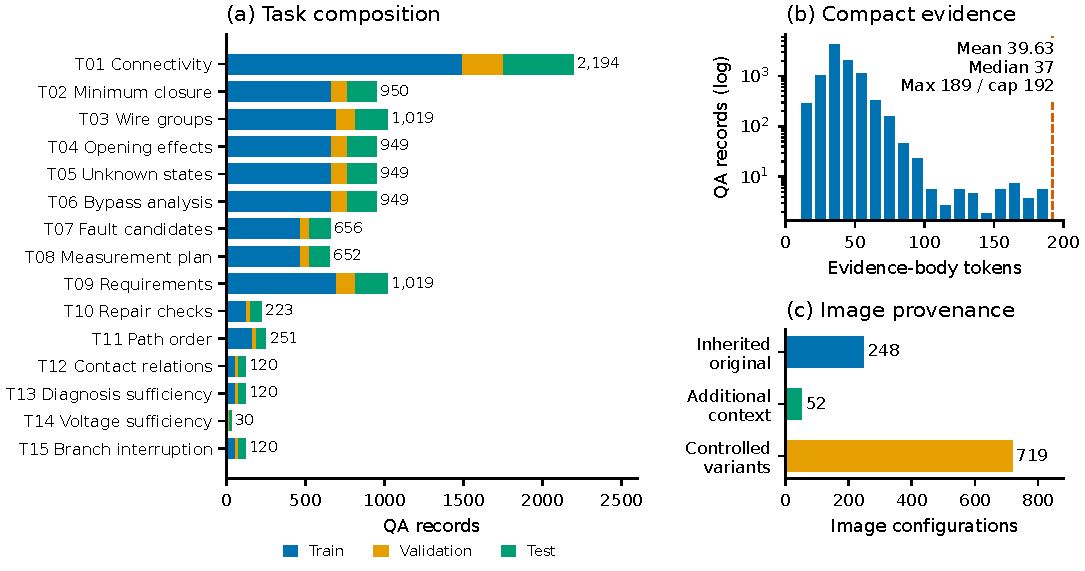
\includegraphics[width=\textwidth]{assets/figure_04.pdf}
\caption{Composition of the ELEC-VQA dataset: (a) QA by task and split; (b) evidence-body length under the local Qwen tokenizer, with logarithmic count scale and a 192-token cap; and (c) image provenance. Original windows may overlap within a drawing; controlled variants retain their parent-window identities.}
\label{fig:distribution}
\end{figure*}

\subsection{Interventions, Verification, and Partitions}
The 719 controlled variants include omitted wires, contact bypasses, wrong rewirings, and cross-network links. They are synthetic edits, not observed field-fault frequencies. Tasks are instantiated under explicit contact-state assignments and fault assumptions, with candidate questions retained only when their reference outcomes and evidence satisfy the corresponding verification queries.

The release audit replays 50,630 graph queries and checks training-view alignment, semantic-specification duplicates, file hashes, and split membership. The duplicate test compares task parameters and verification conditions within an image/task; it does not establish complete conceptual novelty or graph-isomorphism independence. Source rendering audits additionally check image decoding and geometry consistency. These checks establish consistency with the extracted representation, not independent expert correctness. A shared extraction error can survive graph replay.

Training, validation, and test contain 6,972, 1,155, and 2,074 QA over 697, 122, and 200 images, respectively. All source projects, DWGs, and parent families are disjoint across splits. Overlapping context windows and related variants remain grouped, but electrically similar templates may occur in different projects. Reporting follows the principle that composition, provenance, and reuse conditions should be documented explicitly~\cite{gebru2021datasheets}. The construction audit and independent reference-quality assessment are distinguished in Section~\ref{sec:experiments}.

\section{Evidence-Guided Adaptation and Evaluation}\label{sec:protocol}
\subsection{Aligned Supervision Views}
For image $I_i$, question $q_i$, short answer $a_i$, and compact evidence $e_i$, the two principal targets are
\begin{equation}
y_i^A=a_i,\qquad y_i^E=\texttt{Evidence: }e_i\;\texttt{Answer: }a_i.
\label{eq:targets}
\end{equation}
The views retain identical record IDs, input questions, images, and final answers. Reference graphs, source-edit labels, typed results, and expected evidence are not appended to model inputs. Consequently, a difference between the two adapters concerns the tested supervision recipe, rather than access to additional inference-time annotations. Figure~\ref{fig:supervision} illustrates the input/output comparison. In the illustrated continuity-test case, either of two series-contact faults explains the failed observation. The compact certificate names both candidates and their shared observable consequence, exposing the distinction between fault compatibility and unique diagnosis. This supervision is intended to teach electrically relevant alternatives and the limits of available information, rather than only a binary label. Its utility is tested through answer correctness and evidence validity; improvement over answer-only training is not assumed.

\begin{figure*}[t]
\centering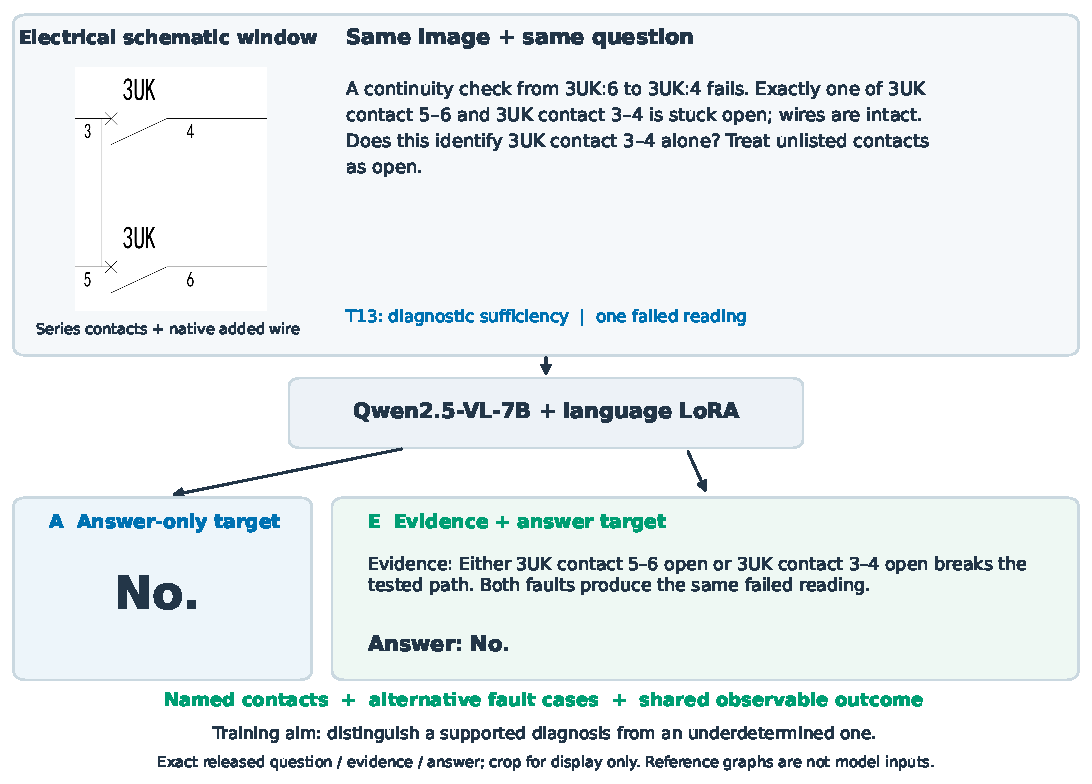
\includegraphics[width=\textwidth]{assets/figure_05.pdf}
\caption{Aligned supervision illustrated by a diagnostic-sufficiency example from the ELEC-VQA dataset. The same image and exact released question lead to either the short answer (A) or the released compact evidence followed by the same answer (E). The evidence identifies two distinct contact faults that produce the same failed continuity reading. Targets are reference annotations, not model predictions; the screenshot is cropped only for display. Equal examples and epochs do not imply equal token exposure or computation.}
\label{fig:supervision}
\end{figure*}

The backbone is Qwen2.5-VL-7B-Instruct~\cite{bai2025qwen}. Standard LoRA~\cite{hu2021lora} updates language attention query, key, value, and output projections; pretrained backbone and vision weights remain frozen. The assistant-token objective is
\begin{equation}
\mathcal L=-\sum_i\sum_{t\in\mathcal A_i}\log p_\theta(y_{i,t}\mid I_i,q_i,y_{i,<t}),
\label{eq:loss}
\end{equation}
where $\mathcal A_i$ excludes user, image, and padding positions. All assistant target tokens receive equal loss weight. Because the evidence target is longer, equal epochs do not imply equal supervised-token exposure or computation.

Fine-tuning uses BF16, rank 16, scaling 32, dropout 0.05, learning rate $10^{-4}$, three epochs, microbatch one, and gradient accumulation eight. Image area and context length are capped at 2,097,152 pixels and 8,192 tokens. The slow Qwen processor and scaled dot-product attention are fixed. Runs use Ubuntu 22.04 and one NVIDIA H100 GPU. The primary comparison uses seed 42 and the final-epoch adapters. Table~\ref{tab:training} summarizes the training settings.

\begin{table*}[t]
\centering\small
\caption{Matched training configuration for answer-only and compact-evidence fine-tuning.}
\label{tab:training}
\begin{tabularx}{\textwidth}{@{}XXX@{}}\toprule
Setting & Answer only & Evidence--answer \\\midrule
Backbone & Qwen2.5-VL-7B-Instruct & Qwen2.5-VL-7B-Instruct \\
Training QA / images & 6,972 / 697 & 6,972 / 697 \\
Target format & Short answer & Compact evidence, then answer \\
Adapted projections & Language $q,k,v,o$ & Language $q,k,v,o$ \\
LoRA rank / scaling / dropout & 16 / 32 / 0.05 & 16 / 32 / 0.05 \\
Precision / attention & BF16 / SDPA & BF16 / SDPA \\
Learning rate / schedule & $10^{-4}$ / cosine & $10^{-4}$ / cosine \\
Epochs & 3 & 3 \\
Microbatch / accumulation & 1 / 8 & 1 / 8 \\
Maximum pixels / context tokens & 2,097,152 / 8,192 & 2,097,152 / 8,192 \\
Processor / primary seed & Slow / 42 & Slow / 42 \\
Checkpoint policy & Final epoch & Final epoch \\
Updates / supervised tokens & \pending & \pending \\
\bottomrule\end{tabularx}
\end{table*}

\subsection{Reference-Guided Semantic Assessment}
Surface-form exact match is insufficient for comparing free-form baseline responses with adapters trained on concise targets. A correct decision need not begin with a fixed prefix, whereas an almost identical sentence can reverse a contact state or terminal relation. We therefore specify a common reference-guided judge, inspired by LAVE~\cite{manas2024lave}, for every compared model. Each request contains the exact question, the complete unmodified response, the reference short answer, a fixed task rubric, and a deterministic reference-fact package. The package includes typed results, relevant task parameters, labeled nodes and edges, and verification queries. These are evaluation-side annotations; the tested VQA model receives only its image and question. The judge is not asked to independently reinterpret the screenshot.

Ratings concern whether the final answer satisfies the electrical task, rather than resemblance to the reference wording. The task rubric preserves terminal identities, negation, explicit conditions, set completeness, and path order; alternative valid minimum plans or conducting routes are admissible. A solution that cannot be established from the reference specification remains unresolved. The same request construction and rubric apply to Base, A, E, and cross-family baselines. 

Let $r_i\in\{1,2,3,\bot\}$ be the judge rating, where 3 denotes a fully correct answer, 2 an explicitly correct but incomplete answer when permitted by the task rubric, 1 an incorrect or absent answer, and $\bot$ an unresolved evaluation. For resolved responses, the auxiliary semantic score is
\begin{equation}
s_i=(r_i-1)/2,\qquad c_i=\mathbb{1}[r_i=3].
\label{eq:judgescore}
\end{equation}
Only full credit contributes to the primary accuracy. Binary decisions, three-way state classification, and a single relation category do not receive partial credit. Evaluator uncertainty is not a score of $0.5$. With $\mathcal R$ the resolved subset of an $N$-question panel, unresolved evaluations give the reporting bounds
\begin{equation}
 A^-={\textstyle\sum_{i\in\mathcal R}c_i\over N},\qquad
 A^+=A^-+{N-|\mathcal R|\over N}.
\label{eq:unresolvedbounds}
\end{equation}
These bounds describe the original automatic-only sensitivity analysis; the provisional supplementary scoring in Section~\ref{sec:experiments} is reported separately. They are missing-judgment bounds, not statistical confidence intervals. Coverage is $|\mathcal R|/N$; mean semantic scores retain the same full-panel denominator and analogous bounds. Empty answers and clearly wrong decisions remain model failures, rather than being removed as unresolved cases.

Answer and evidence assessments are separated. Additional explanatory tokens neither earn answer credit nor incur a length penalty. A correct final answer with an invalid explanatory detail can receive answer credit but fails evidence or joint correctness; an unresolved contradiction in the final decision cannot be repaired by selecting its favorable sentence. Primary reporting uses QA-micro full-credit accuracy and equal-weight task macro accuracy over 14 families. T14's ten all-negative test questions are reported separately, leaving 2,064 questions in the primary held-out panel. Source-DWG macro accuracy and all-15-task results retain their explicit denominators. Reference quality and evaluator uncertainty limit the reliability of these automatic ratings~\cite{zheng2023judge,zeng2024llmbar}.

\subsection{Controlled-Change and Evidence Metrics}
Visual pairs use identical questions on different images, whereas condition pairs use the same image with a changed contact-state assumption. The pair audit checks question identity and reference outcomes, retaining both outcome-flip and invariant pairs.

For an admissible pair set $\mathcal P$, both responses must receive full credit; write $S_i=c_i$ for resolved judgments:
\begin{equation}
A_{\rm pair}=\frac{1}{|\mathcal P|}\sum_{(i,j)\in\mathcal P}S_i(\hat a_i)S_j(\hat a_j).
\label{eq:pair}
\end{equation}
An answer change alone does not establish successful change-sensitive reasoning: both predictions must satisfy their respective conditions. Pair statistics preserve the shared source identity and distinguish outcome-flip from invariant cases. The test inventory contains seven DWGs from two projects, limiting inferences about broader industrial populations.

Evidence is assessed for entity grounding, route or blocking-fact validity, compliance with stated conditions, treatment of necessary alternatives, and support for the answer. Joint correctness requires both a correct answer and valid evidence. Alternative valid certificates are accepted rather than matched verbatim. These criteria concern the observable explanation, not faithfulness to hidden computation~\cite{deyoung2020eraser,turpin2023unfaithful}.

\subsection{Common Inputs and Inference Budgets}
The controlled comparison contains the unchanged backbone (Base), the answer-only adapter (A), and the evidence--answer adapter (E). InternVL2\_5-8B and LLaVA-OneVision Qwen2 7B provide cross-family zero-shot context~\cite{internvl25card,llavaonevisioncard,li2024onevision}. Every comparator receives the same image and question under its native processor. Pixel budgets, tiling, visual tokens, checkpoint revisions, and prompts are logged; native processing is not described as pixel-identical preprocessing.

Two prompt tracks isolate answer ability from requested explanation. The main track appends ``Give a brief answer in English. Do not include an explanation.'' to the same released question for every comparator. A separate evidence-request track asks for relevant visible components, connections and conditions, followed by an \texttt{Answer:} line, for Base/A/E. Both tracks preserve the complete response for judging; the requested format is not a scoring criterion. Greedy decoding and a 768-new-token ceiling are checked on validation and frozen before test, with any truncation-driven revision documented. Text-only models supplied with netlists constitute a separate assisted-input condition, whereas text-only judges act solely on the evaluation side.
\section{Experiments and Comparative Study}\label{sec:experiments}
\researchquestion{RQ1}{Cross-model understanding}{How do general-purpose vision--language models perform on ELEC-VQA?}
\researchquestion{RQ2}{Domain adaptation}{How do answer-only and evidence--answer supervision interact with output prompting?}
\researchquestion{RQ3}{Verifiable evidence}{When does evidence supervision improve supported answers?}
\subsection{Experimental Protocol and Metrics}
The dataset contains 6,972 training, 1,155 validation and 2,074 test QA records. Excluding ten T14 diagnostic controls per evaluation split gives 1,145 validation and 2,064 test questions. The test panel spans seven source DWGs from two projects. Questions and variants sharing a source remain statistically dependent.
The comparators are Qwen2.5-VL-7B-Instruct (Base), its answer-only adapter A, its compact-evidence--answer adapter E, InternVL2\_5-8B and LLaVA-OneVision Qwen2 7B. Adapters use seed 42. Models receive identical questions and raw images with native preprocessing. Greedy decoding allows 768 new tokens. The direct track requests a brief answer without explanation. A second track requests visible components, connections and conditions, followed by a brief final answer, identically for Base/A/E.

Qwen2.5-32B-Instruct is the sole automatic judge. Reference-guided absolute grading follows LAVE~\cite{manas2024lave}; prior Qwen judge evaluations provide precedent~\cite{yu2025risejudge}, not domain-specific validation. Model identities are withheld. Responses receive ratings 3 (full), 2 (task-permitted partial), or 1 (no credit), mapped to semantic scores 1, 0.5 and 0. Binary decisions receive no partial credit. A correct short answer requires no explanation for answer credit. Evidence is scored separately for valid entities, paths, states and support. Joint full credit requires answer and evidence ratings of 3 for the same response. Judge inference uses BF16/SDPA, a 12,288-input-token ceiling, 512 new tokens and one format-recovery retry.

The primary tables include provisional, reference-based supplementary ratings for 585 originally unresolved judgments: 28 direct-answer, 75 explanation-track answer and 482 evidence records. These concern 552 responses to 517 questions, not 585 independent questions. Original non-null Qwen ratings remain fixed. Supplementation combines assistant assessment against the released references with recovery of 85 consistent numerical suggestions from original judge attempts. None has independent human confirmation. These are therefore mixed-evaluator provisional results, not fully automatic or expert-validated scores. The unchanged Qwen-only estimates are retained as a sensitivity analysis. Reference and evaluator errors remain limitations~\cite{zheng2023judge}. No sample is removed to improve a score.

We report QA-micro full-credit accuracy, equal-weight task and drawing macro accuracy, and auxiliary semantic score. T14 is diagnostic and excluded from primary aggregates. A paired bootstrap resamples the seven source DWGs with replacement, retaining all their questions (2,000 replicates, seed 42). Intervals quantify source-resampling variability, not judge bias, supplementary-rating validity or training-seed variability.

\subsection{Cross-Model Answer Results}
A achieves 74.27\% direct-answer full credit, exceeding Base by 37.11 percentage points. E reaches 52.42\%, above Base but below A by 21.85 points. Cross-family baselines remain near 34.5\% (Table~\ref{tab:main}). Native preprocessing and pretraining differences prevent interpreting the comparison as an isolated architectural effect.

\begin{table*}[t]\centering\small
\caption{Direct-answer test results (\%). Supplemented denotes originally unresolved ratings assigned provisional scores; it is not a count of additional test samples.}\label{tab:main}
\begin{tabular}{lrrrrr}\toprule Model & Full credit & Task macro & DWG macro & Semantic & Supplemented\\\midrule
A & 74.27 & 74.98 & 59.89 & 75.34 & 3 \\
E & 52.42 & 52.39 & 40.73 & 52.98 & 3 \\
Base & 37.16 & 33.93 & 42.10 & 38.06 & 11 \\
InternVL2.5-8B & 34.45 & 32.83 & 35.66 & 35.47 & 4 \\
LLaVA-OneVision & 34.54 & 32.28 & 30.47 & 35.00 & 7 \\
\bottomrule\end{tabular}\end{table*}
\subsection{Output Prompt and Evidence Supervision}
Under common explanation prompting, answer accuracy is 39.00\% for Base, 70.16\% for A and 67.97\% for E (Fig.~\ref{fig:effects}). E improves by 15.55 points relative to direct mode, with a drawing-cluster bootstrap interval of [12.63,17.86]. A changes by -4.12 points [-4.92,-2.35]. The explanation-track A-minus-E gap is 2.18 points [-1.61,6.65]. An interval spanning zero establishes neither equivalence nor a stable answer advantage for E. Output alignment and additional generated computation remain alternative explanations; these comparisons do not demonstrate a causal effect of visible reasoning text.

\begin{figure}[t]\centering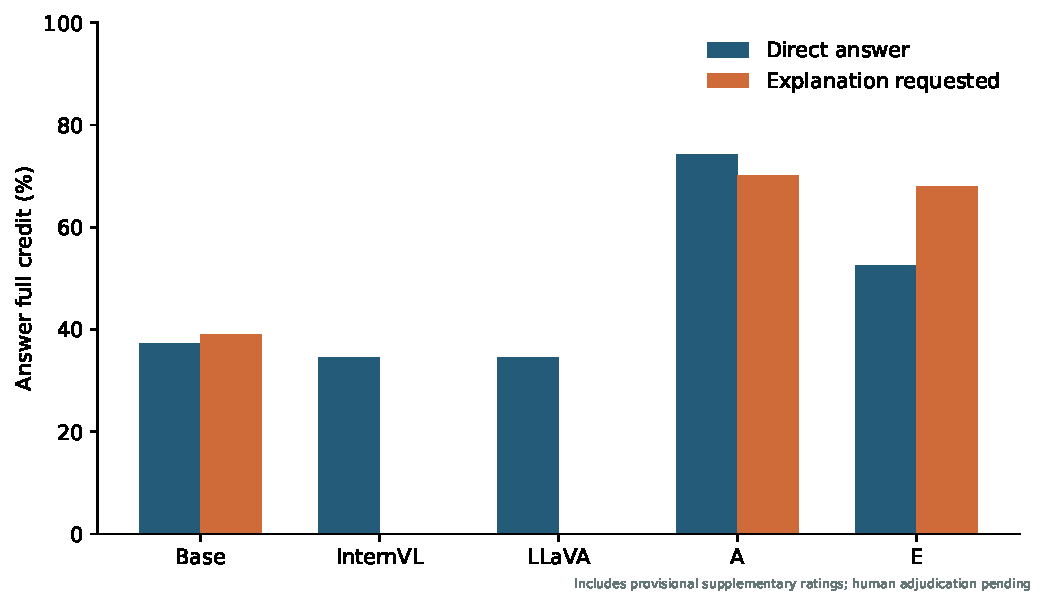
\includegraphics[width=\linewidth]{assets/figure_06.pdf}
\caption{Answer full credit under the two output protocols. Explanation tracks are evaluated for Base/A/E only.}\label{fig:effects}\end{figure}
\subsection{Evidence and Joint Correctness}
E achieves 64.78\% evidence full credit and 64.24\% joint full credit, compared with A's 46.27\% and 46.17\%. The joint improvement is 18.07 points, with a drawing-cluster bootstrap interval [16.04,20.44]. This supports improved reference-supported responses rather than uniformly better final decisions.

\begin{table}[t]\centering\small
\caption{Common explanation-track full credit (\%), including provisional supplementary ratings.}\label{tab:evidence}
\begin{tabular}{lrrr}\toprule Model & Answer & Evidence & Joint\\\midrule
Base & 39.00 & 32.17 & 31.93 \\
A & 70.16 & 46.27 & 46.17 \\
E & 67.97 & 64.78 & 64.24 \\
\bottomrule\end{tabular}\end{table}
A sensitivity analysis with supplementary judgments withheld gives original Qwen-only joint lower estimates are 46.08\% for A and 63.76\% for E; the corresponding unresolved upper bounds are 63.18\% and 64.78\%. Thus, the original E lower estimate exceeds A's original upper bound by 0.58 points within missing-rating assignments. This does not protect against systematic reference or judge error. Original direct-answer estimates are 74.18\% for A and 52.37\% for E, compared with the supplemented values in Table~\ref{tab:main}. The central ordering is preserved.

\begin{figure}[t]\centering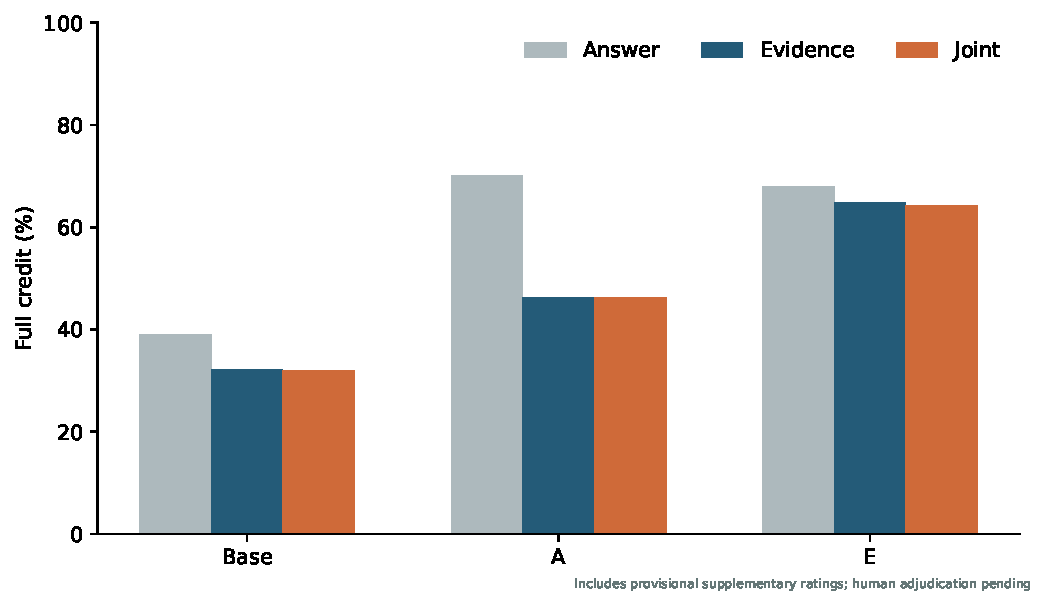
\includegraphics[width=\linewidth]{assets/figure_07.pdf}
\caption{Answer, evidence and joint full credit with common explanation prompting.}\label{fig:evidence}\end{figure}
\subsection{Conditions Under Which E Outperforms A}
E improves answer full credit on measurement planning (T08, +42.52 points), diagnosis sufficiency (T13, +15.00), open-contact impact (T04, +6.63), branch interruption (T15, +7.50) and contact order (T11, +5.26). Conversely, minimum closure, wire grouping and hypothetical bypass remain weaker. Table~\ref{tab:pertask} reports every primary family. Differences are exploratory and are not adjusted for multiple comparisons.
\begin{table}[t]\centering\small
\caption{E minus A under identical explanation prompting (percentage points).}\label{tab:pertask}
\begin{tabular}{lrrr}\toprule Task & N & Answer difference & Joint difference\\\midrule
T01 & 440 & -5.68 & +38.64 \\
T02 & 181 & -9.39 & -13.81 \\
T03 & 200 & -12.50 & -13.50 \\
T04 & 181 & +6.63 & +30.94 \\
T05 & 181 & -5.52 & -4.97 \\
T06 & 181 & -14.36 & -4.97 \\
T07 & 127 & -3.94 & -6.30 \\
T08 & 127 & +42.52 & +44.88 \\
T09 & 200 & -2.00 & +46.50 \\
T10 & 69 & -11.59 & +21.74 \\
T11 & 57 & +5.26 & +7.02 \\
T12 & 40 & -7.50 & +10.00 \\
T13 & 40 & +15.00 & +80.00 \\
T15 & 40 & +7.50 & +50.00 \\
\bottomrule\end{tabular}\end{table}
An original-DWG case asks whether bridging open 2ZJ contact 24--23 connects 3UK:4 to CZ:41 while 3UK contact 3--4 is closed. Both adapters fail under direct prompting; A also fails when explanation is requested. E identifies the visible route 3UK:4 $\rightarrow$ 3UK:3 $\rightarrow$ 2ZJ:24 $\rightarrow$ 2ZJ:23 $\rightarrow$ CZ:41 and answers correctly. This illustrates successful explicit decomposition, not an intervention on internal reasoning.

\begin{figure}[t]\centering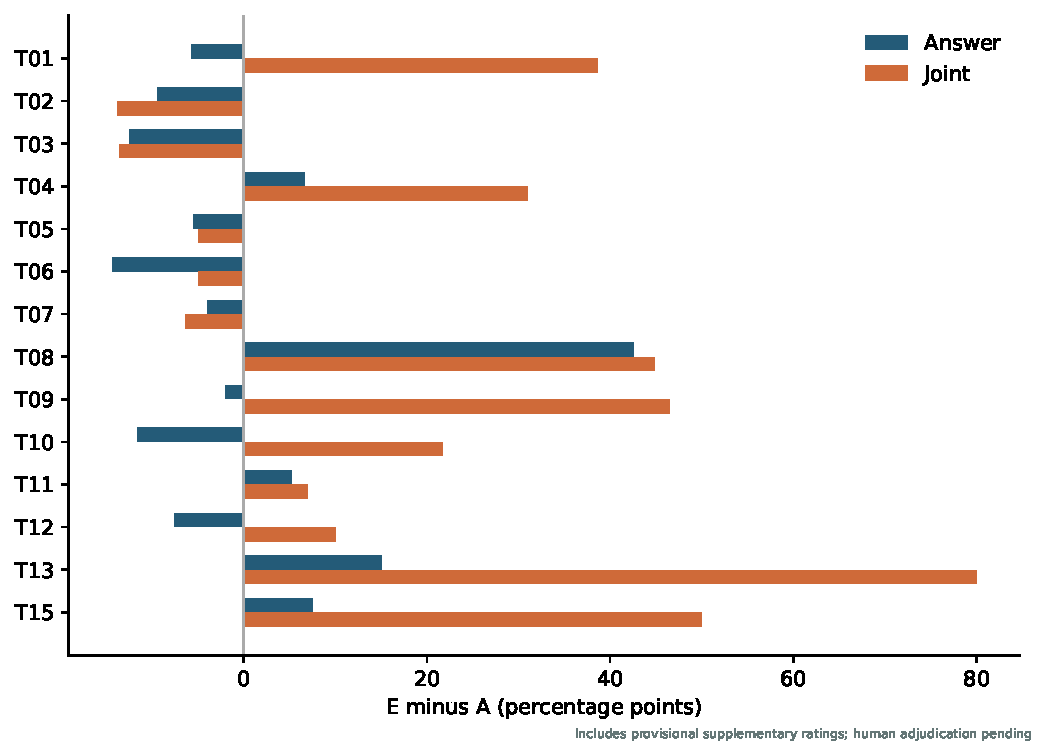
\includegraphics[width=\linewidth]{assets/figure_08.pdf}
\caption{Task-dependent gains and losses for E. All primary families are retained.}\label{fig:taskeffects}\end{figure}
\subsection{Conditional Support and the Answer--Evidence Gap}
Following the distinction between task performance and explanation quality in e-ViL~\cite{kayser2021evil}, let $C_i$ indicate answer full credit and $V_i$ evidence full credit. Conditional support is
\begin{equation}
Q_{E\mid A}=\frac{\sum_i C_iV_i}{\sum_i C_i}.
\end{equation}
The denominator contains correct answers, unlike joint accuracy, which uses the complete question panel. The metric assesses observable support rather than causal faithfulness; sufficiency and comprehensiveness~\cite{deyoung2020eraser} require input interventions and new predictions and are not inferred here.
Conditional support is 65.81\% for A and 94.51\% for E. Accordingly, 34.19\% and 5.49\% of correct answers lack full-credit evidence. This gap indicates that a correct conclusion can coexist with absent, incomplete or incorrect support; those categories should not all be called hallucination. Base attains 81.86\%, but answers fewer questions correctly, so a high conditional value does not imply stronger overall supported reasoning. Conditioning on correct answers also changes the selected subset across models.

\begin{figure}[t]\centering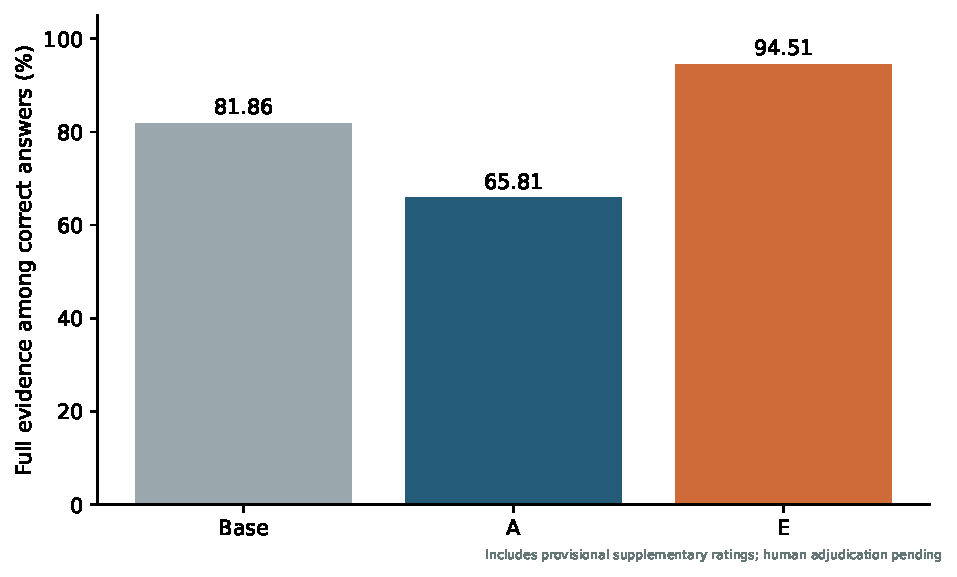
\includegraphics[width=\linewidth]{assets/figure_09.pdf}
\caption{Full-credit evidence conditional on answer full credit, using supplemented ratings.}\label{fig:conditional}\end{figure}
\subsection{Sensitivity to Controlled Changes}
Motivated by consistency analysis in GQA~\cite{hudson2019gqa}, a pair succeeds only when both answers receive full credit; merely changing an output is insufficient. The fixed inventory comprises 69 visual and 179 state pairs. Shared questions and circuits preclude treating them as independent trials.

Under common explanation prompting, E succeeds on 77/82 state-flip pairs (93.90\%) versus A's 55/82 (67.07\%). However, E succeeds on only 11/97 state-invariant pairs (11.34\%) versus A's 60/97 (61.86\%). E improves on visual-invariant pairs (40/46, 86.96\%, versus 36/46, 78.26\%), but is weaker on visual-flip pairs (1/23, 4.35\%, versus 9/23, 39.13\%). Evidence-guided adaptation is therefore more successful for selected relevant state changes but insufficiently selective for irrelevant changes, and weak for topology-changing visual pairs. Better explanation production does not establish robust visual causal understanding.
\begin{figure}[t]\centering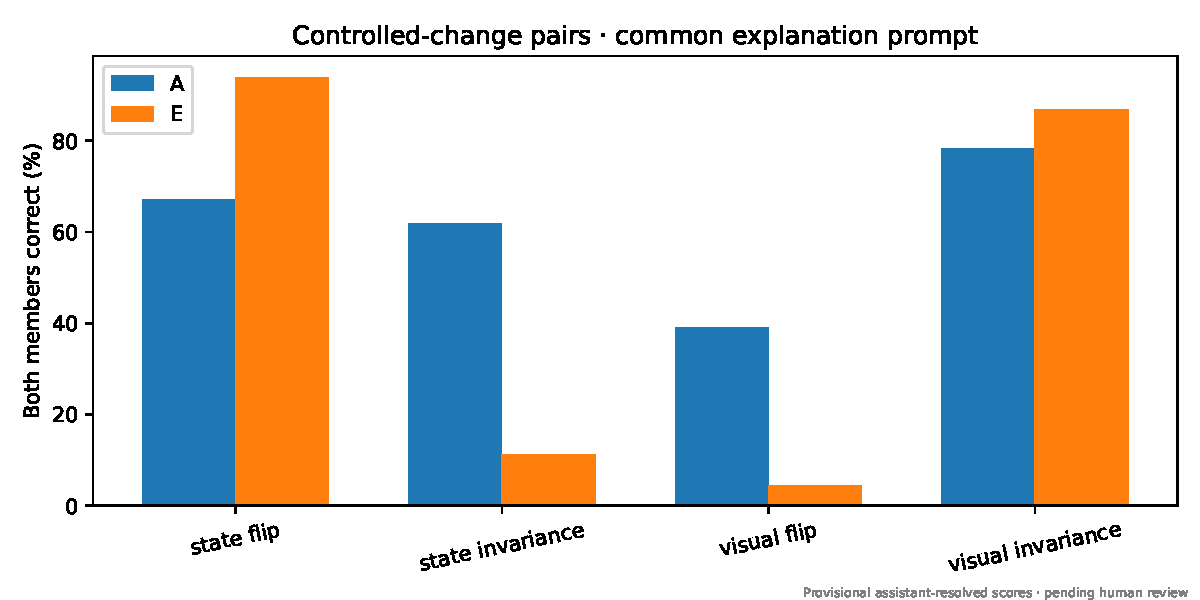
\includegraphics[width=\linewidth]{assets/figure_10.pdf}
\caption{Both-members-correct performance on the fixed change-pair inventory.}\label{fig:pairscores}\end{figure}
\subsection{Reference Complexity and Heterogeneous Gains}
On the 98 questions with at least three explicit reference states, E achieves 63.27\% answer full credit versus 43.88\% for A, a 19.39-point advantage. On the 1,445 two-state questions, they are close (73.08\% versus 73.63\%); E is worse on one-state questions (56.24\% versus 69.58\%). E also exceeds A on recorded paths of four to six edges (61.81\% versus 58.32\%) and seven or more edges (53.00\% versus 49.77\%).

Edge counts concern the bounded reference graph, not visible wire segments or latent reasoning steps. Questions without a recorded path form a separate group. Task composition, answer distribution and complexity are correlated; these exploratory strata do not isolate a causal complexity effect. The findings support improved explicit justification and selective conditional reasoning, alongside topology and relevance failures.
\begin{figure*}[t]\centering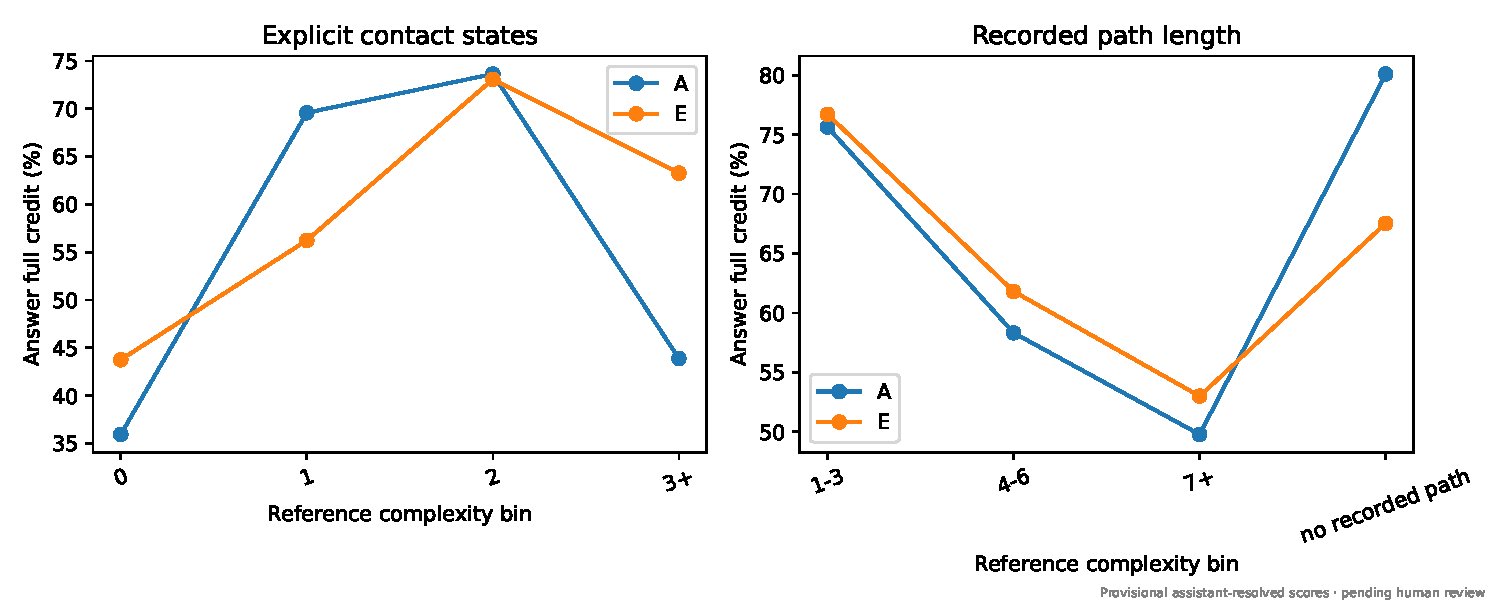
\includegraphics[width=.85\textwidth]{assets/figure_11.pdf}
\caption{Answer full credit by reference-state count and maximum recorded path length. All bins are retained.}\label{fig:complexity}\end{figure*}
\subsection{Generation Cost and Limitations}
Direct-track mean generation times are 0.65, 0.73 and 1.21 seconds for Base, A and E; explanation prompting increases these to 6.67, 0.82 and 2.30 seconds. Mean generated explanation-track lengths are 278.13, 13.10 and 54.81 tokens. A remains brief despite the evidence request. E's evidence advantage incurs additional generation cost. These per-response latencies are not deployment throughput or a hardware-normalized architectural comparison. Efficiency summaries retain all 2,074 test responses, including T14, whereas accuracy aggregates exclude T14.
\begin{figure}[t]\centering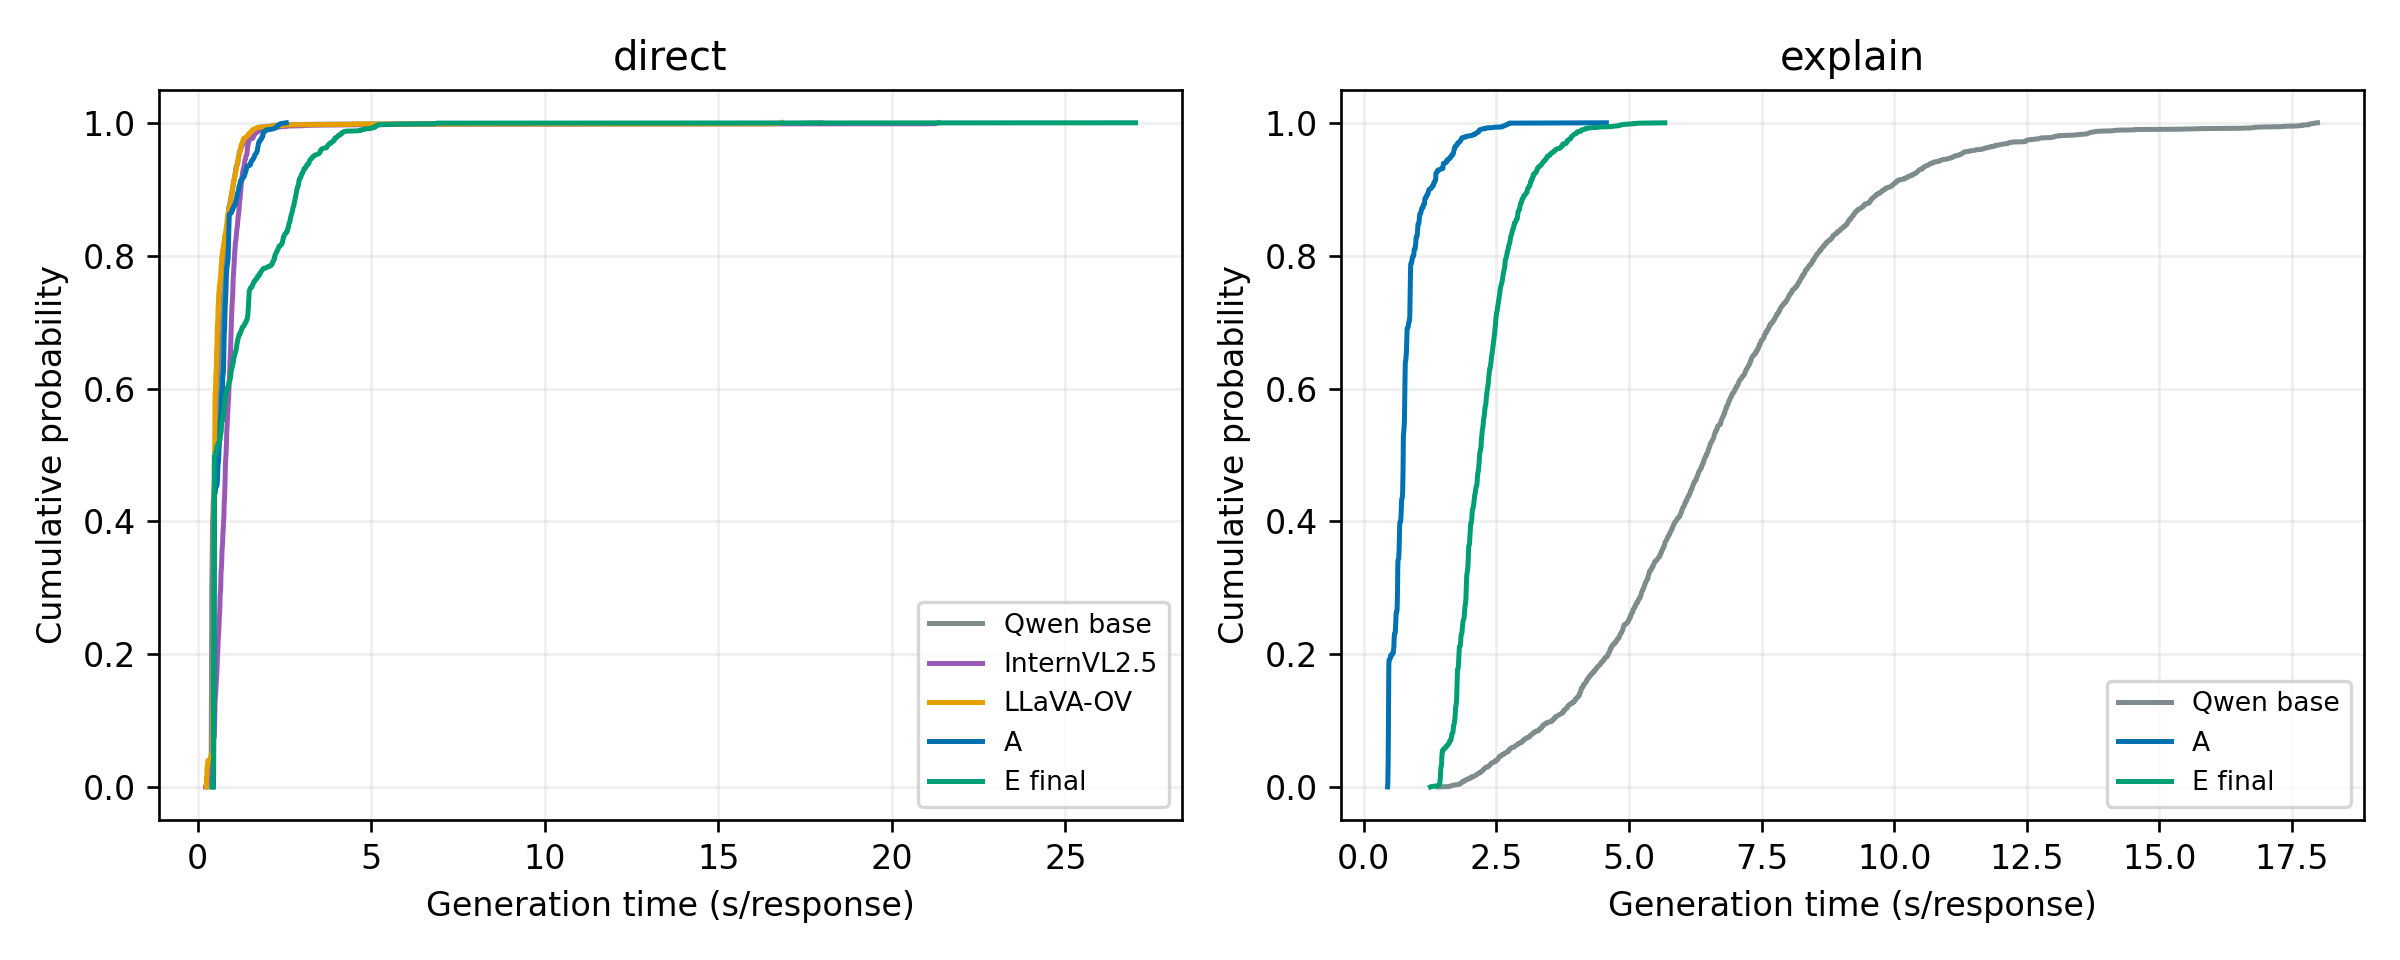
\includegraphics[width=\linewidth]{assets/figure_12.png}
\caption{Generation-latency distributions under the two output protocols.}\label{fig:latency}\end{figure}
The study uses one training seed, seven held-out drawings and references without independent expert validation. Provisional supplementary scoring introduces additional evaluator uncertainty. Domain-adaptation gains and improved supported output are observed within this scope; universal superiority, causal reasoning faithfulness and broad industrial generalization are not established.

\section{Representative Cases and Discussion}\label{sec:discussion}
\subsection{Dataset Cases as Verifiable Reasoning Examples}
The appendix presents six examples from different original DWG windows, covering minimum closure, wire grouping, unknown contact states, fault diagnosis, path order, and branch interruption (Figs.~\ref{fig:appendix1}--\ref{fig:appendix3}). They illustrate annotation semantics rather than held-out model performance.

The examples distinguish three sources of electrical difficulty. First, wire-only grouping differs from continuity through closed contacts: a model must identify which edges depend on the stated operating conditions. Second, fault diagnosis requires comparing predicted observations across hypotheses, rather than merely locating a broken-looking contact. Third, a state change can be irrelevant to the queried branch, so interruption questions require tracing the actual path instead of associating every switch with every nearby terminal. Compact evidence makes these distinctions explicit through a route, a counterexample, or a short observation signature.

\subsection{Interpreting Evidence Effects}
Answer-only supervision produces the strongest direct-answer accuracy. Under common explanation prompting, E instead achieves higher confirmed evidence and joint correctness, with answer advantages concentrated in measurement planning, diagnosis sufficiency and selected state-dependent tasks. These gains coexist with losses in minimum closure, grouping and bypass questions. Evidence supervision is therefore useful when supported justifications are required, but is not uniformly superior.

The original-DWG path example illustrates a successful explicit decomposition. Neither this case nor the aggregate prompt interaction proves causal faithfulness of generated text. Longer training targets, output alignment and evaluator artifacts remain alternative explanations. The fixed-seed study cannot isolate the causal contribution of evidence content.

\subsection{Scope, Dependence, and Annotation Limitations}
The name \dataset describes the task domain; its current empirical coverage is substation secondary wiring, not all electrical schematics. The two held-out projects and 300 partially overlapping original windows limit claims about general industrial transfer. Distinct image hashes and source partitions do not eliminate repeated engineering templates or abstractly isomorphic graphs. Larger or more diverse external sources would be needed for broad cross-domain claims.

The automatic annotation pipeline can produce self-consistent but visually incorrect references if entity extraction is wrong. Source traceability facilitates correction; it does not replace independent review. T12 has no verified parallel cases, T14 has a fixed negative answer prior, and generated question templates may permit shortcuts. These limitations motivate per-task reporting, label-prior controls, and explicit separation of diagnostic tasks. Native edits represent controlled perturbations rather than realistic fault prevalence or validated maintenance procedures.

\subsection{Implications for Schematic Understanding}
The results favor a distinction between concise decision support and evidence-backed interpretation. Compact evidence supervision improves the availability of valid justifications and selected multi-condition tasks, while answer-only supervision remains preferable for overall direct-answer accuracy. The state-invariance and visual-flip failures reveal that successful explanation generation is not sufficient for selective use of electrical conditions or robust perception of altered topology. A useful next step is evidence supervision that explicitly contrasts relevant and irrelevant changes, evaluated across additional drawing sources and repeated training seeds.

\FloatBarrier
\section{Conclusion}\label{sec:conclusion}
ELEC-VQA combines 10,201 engineering QA records, 1,019 schematic configurations, compact evidence and source-disjoint evaluation. The comparative study, including provisional supplementary adjudication, demonstrates substantial domain-adaptation gains, but distinguishes answer accuracy from supported reasoning. Answer-only adaptation achieves the strongest concise-answer result; evidence-guided adaptation yields higher joint correctness and more reliable support conditional on correct answers. Gains concentrate on measurement planning and selected multi-condition tasks. Controlled-change pairs expose complementary failures in irrelevant-state invariance and visual topology sensitivity. These results motivate evidence supervision that models both relevant and irrelevant electrical changes, rather than assuming that longer explanations universally improve understanding. Broader drawing coverage, independent reference validation and multiple training seeds are needed to establish generality.

\section*{Data Availability}
The accompanying ELEC-VQA materials comprise schematic images, source-grouped annotations, aligned supervision files, controlled-change pairs, and evaluation code. The dataset is available under CC BY 4.0 and the original project code under the MIT License; third-party materials retain their respective terms.

\appendices
\section{Supplementary Dataset Examples and Structural Coverage}\label{app:contract}
\subsection{Examples from Original Schematic Windows}
Figures~\ref{fig:appendix1}--\ref{fig:appendix3} show six training examples drawn from six different original DWG windows, with no controlled wiring edits. None reuses a screenshot displayed in the main text. Questions and short answers retain the released wording; concise evidence summaries highlight the corresponding graph checks. These examples document dataset content, not model predictions or observed field faults. The examples retain their original source associations.

\begin{figure*}[p]
\centering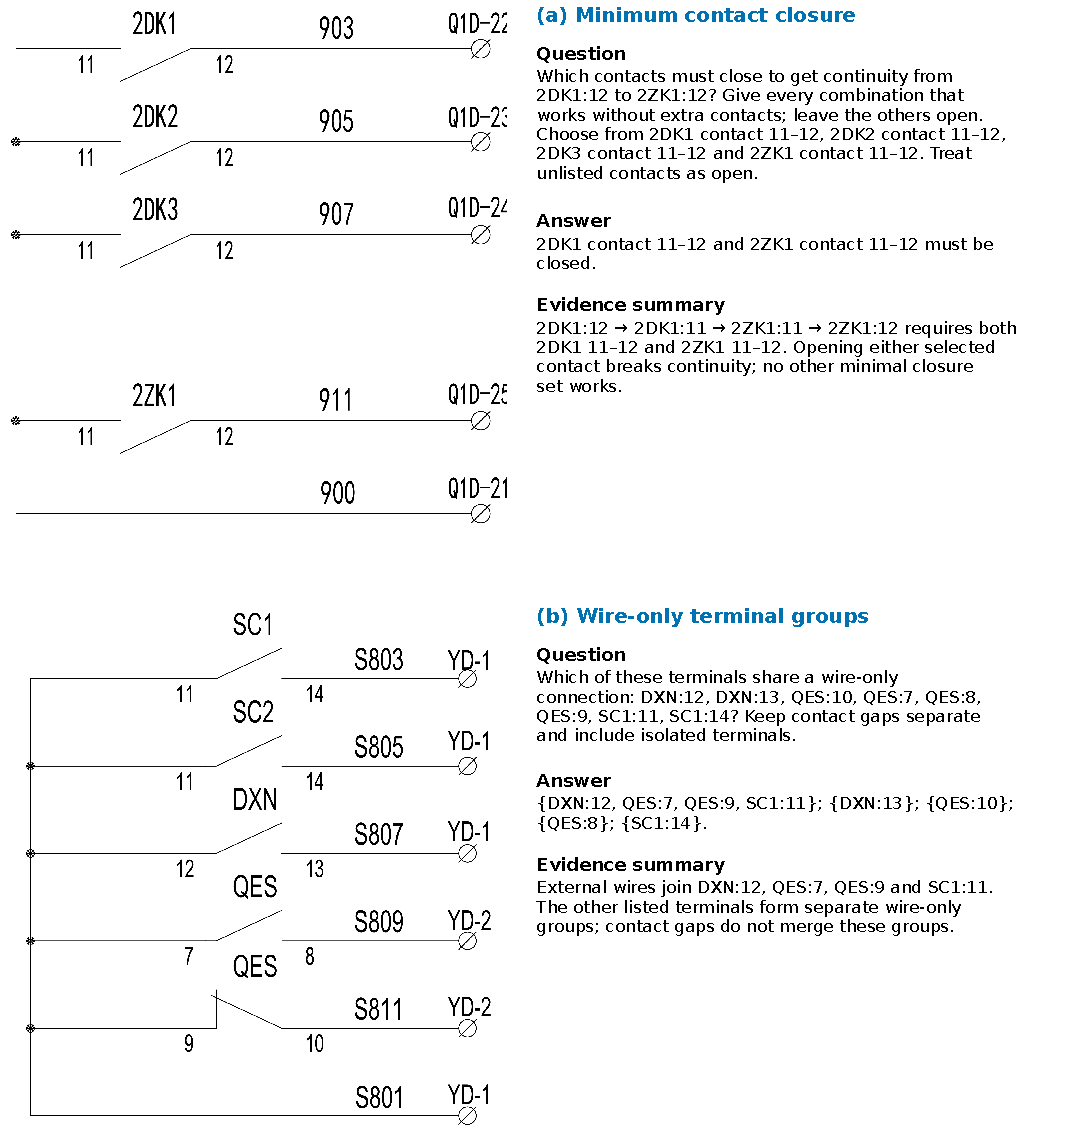
\includegraphics[width=.98\textwidth]{assets/figure_13.pdf}
\caption{Minimum contact closure and wire-only terminal grouping. Contact conduction is governed by the stated assumptions, whereas wire groups exclude contact edges.}
\label{fig:appendix1}
\end{figure*}

\begin{figure*}[p]
\centering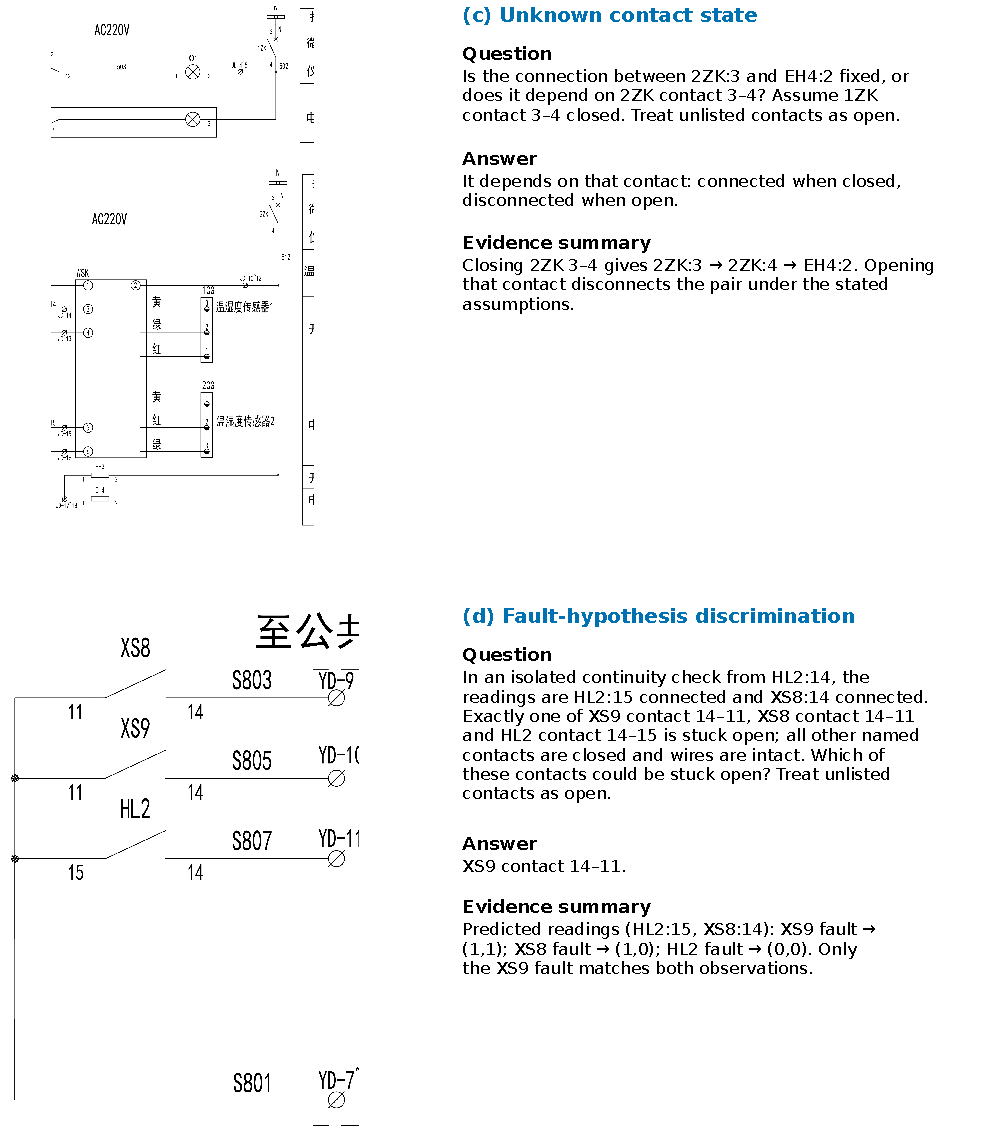
\includegraphics[width=.98\textwidth]{assets/figure_14.pdf}
\caption{State dependence and fault-hypothesis discrimination. Different contact states and fault hypotheses are checked against their corresponding continuity outcomes.}
\label{fig:appendix2}
\end{figure*}

\begin{figure*}[p]
\centering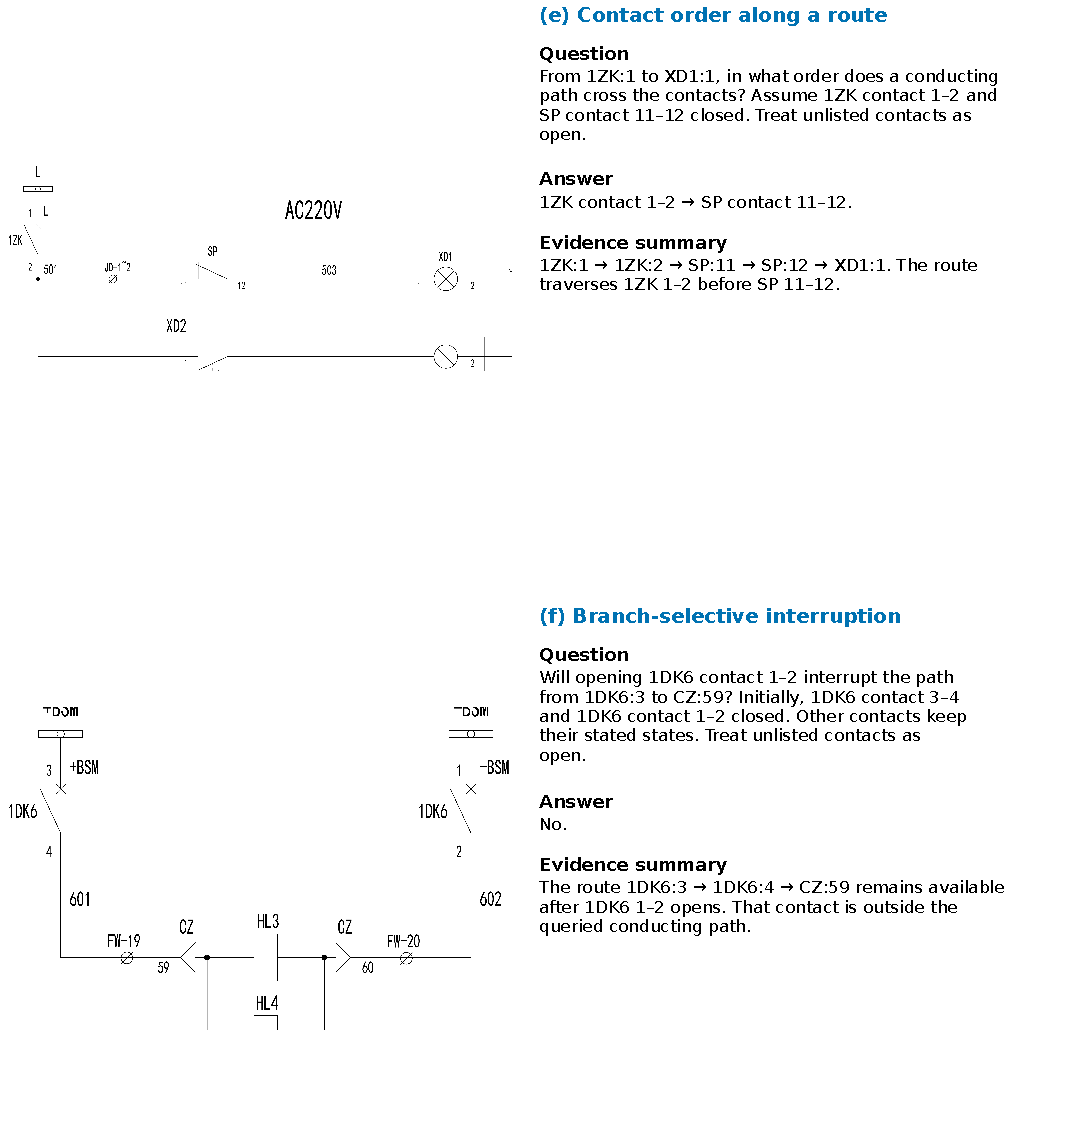
\includegraphics[width=.98\textwidth]{assets/figure_15.pdf}
\caption{Contact order and branch-selective interruption. A valid route identifies the traversed contacts; an unrelated contact opening leaves the queried branch connected.}
\label{fig:appendix3}
\end{figure*}

\subsection{Annotation and Evaluation Records}
Each annotation contains a question, short answer, compact evidence, typed result, task parameters, and source provenance. Verification queries store contact states, graph modifications, connectivity outcomes, and supporting paths or reachable regions. The two training views serialize the same image--question records with different supervision targets; they do not increase the number of distinct QA examples.

Answer and evidence quality are evaluated separately with a three-level electrical rubric. Unresolved judgments are retained, and joint correctness requires both dimensions to receive full credit for the same response.

\subsection{Structural Coverage and Pair Inventory}
Figure~\ref{fig:structure} summarizes the bounded reference graphs for the 300 original context windows, excluding edited variants. These are graph-level counts, not an inventory of every component visible in each screenshot. Table~\ref{tab:pairinventory} records the completed binary pair audit. The inventory is restricted to binary decisions with revalidated outcomes.

\begin{figure*}[t]
\centering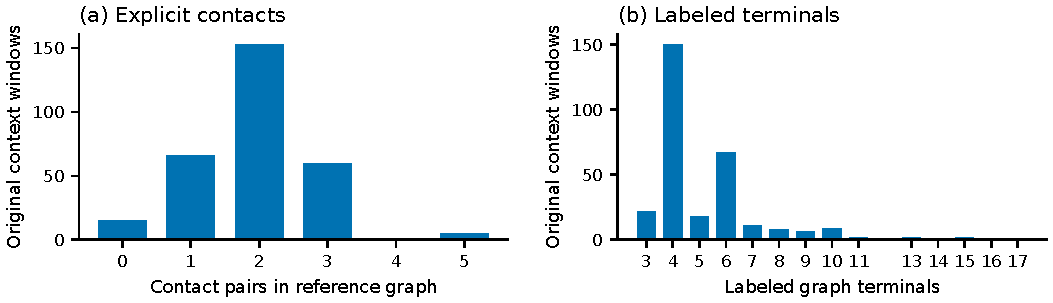
\includegraphics[width=.95\textwidth]{assets/figure_16.pdf}
\caption{Structural coverage of the bounded reference graphs in original contexts. Original windows may overlap within a drawing; graph statistics do not imply independent circuit designs.}
\label{fig:structure}
\end{figure*}

\begin{table}[t]
\centering\small\setlength{\tabcolsep}{3pt}
\caption{Revalidated binary pair inventory. Counts reuse existing QA and are not model scores.}
\label{tab:pairinventory}
\begin{tabularx}{\linewidth}{@{}Xrrrr@{}}\toprule
Split & Visual flip & Visual invariant & State flip & State invariant \\\midrule
Train & 79 & 178 & 340 & 283 \\
Validation & 13 & 23 & 37 & 58 \\
Test & 23 & 46 & 82 & 97 \\
\bottomrule\end{tabularx}
\end{table}

\FloatBarrier
\bibliographystyle{IEEEtran}
\bibliography{references,references_access_additions}
% Insert the confirmed authors' IEEEbiography/IEEEbiographynophoto blocks here.
\EOD
\end{document}
